\documentclass{article}
\usepackage[utf8]{inputenc}
\usepackage{amsmath, amssymb}
\usepackage{hyperref}
\usepackage{graphicx}
\usepackage{caption}
\usepackage{subcaption}

\title{Lotka Volterra Model}
\date{}
\begin{document}

\maketitle

\section{A short introduction}
The Lotka-Volterra model, or the prey predator model is used to model a single prey, single predator ecosystem. If we have $x(t)$ as the prey population and $y(t)$ as the predator population, then this model is governed by the system of differential equations given below :

\begin{equation}
\frac{dx}{dt} = ax - bxy
\end{equation}

\begin{equation}
\frac{dy}{dt} = -cy + dxy
\end{equation}

for positive parameters $a$, $b$, $c$ and $d$.
\\
\\
The rationale behind this is:

\begin{itemize}
\item The prey population, when left unchecked will keep reproducing, since the amount of grass is assumed to be unlimited. The reproduction rate is directly proportional to the population of the prey. But, the predator hunts down the prey, hence they also have a death rate. The death rate will be proportional to the number of interations between the prey and predator, which is assumed to be proportional to their product. Since this term represents death rate, we have the minus sign.

\item The predator population, under the absence of prey to feed upon, will die. Their death rate will be proportional to their population, and hence the $-cy$ term. And, just like in prey, we have the correction term for predators feeding upon the prey. Here, this is suitable to predators as they have a source of food, and hence increases their rate of change. Hence, we have a plus sign, unlike in prey
\end{itemize}



\section{Stability analysis}

\subsection{What is stability?}
Before we answer this, consider a first order differential equation, $$\frac{dx}{dt} = f(x).$$

Now, f(x) itself is a function of x. Let us say $x_0$ is a root of f(x), i.e $f(x_0) = 0$ Consider the constant function $x(t) = x_0$. This horizontal line satisfies our differential equation, since the derivative of a constant function is zero. When we start out with an initial condition $x(t_0) = x_0$, since the derivative of $x$ is zero at $t_0$, $x(t)$ continues to be $x_0$ at a neighborhood. And generalizing, \emph{the initial condition $x(t_0) = x_0$ never moves away from the horizontal line.}

The solution $x(t_0) = x_0$ is called an equilibrium solution, and the point $x_0$ is called fixed point/equilibrium point.

But what about initial conditions \emph{near} $x_0$? They can converge toward the solution $x = x_0$, or move away from it. 

\begin{itemize}
    \item If the system evolves such that $x(t)$ moves further away from $x_0$, i.e if it diverges away, then the fixed point $x = x_0$ is said to be unstable.
    \item If the system evolves in such a way that $x(t)$ comes closer to the fixed point, i.e it converges to the fixed point, then it is said to be stable.
\end{itemize}

This notion of stability is similar to the stability pertaining to the stability of an equilibrium of a body, subject to forces.
\\
\\
Formally, the solution $x = x(t)$ is stable, if for every function $g(t)$ that is close to $x(t)$ at $t = 0$, remains to be closer for all future intervals. In a more rigorous footing, for every $\epsilon > 0$, we have a $\delta > 0$, such that $|g(t) - x(t)| < \epsilon$, whenever $|g(0) - x(0)| < \delta$, and if atleast one such $g(x)$ doesn't follow this, then the solution is unstable. This criteria is called \emph{Lyapunov stability} and the solutions which uphold this criteria are said to be \emph{Lyapunov stable}.
\\
\\
There is another, more strict version of stability and that is the \emph{asymptotic stability}. A solution is said to be \emph{asymptotically stable}, if it is Lyapunov stable plus, solutions with nearby initial conditions converging to this solution as $t \to \infty$. In our analysis, we refer to Lyapunov stability.


\subsection{The second derivative test : Linearizing our differential equation}

Let $x_0$ be a fixed point, and let us consider a function $x(t)$, which has an initial condition, close to $x_0$. We wish to see if it diverges or converges to $x_0$.
For this, define $\epsilon = x(t) - x_0$.
\\
\\
So, $$\frac{d\epsilon}{dt} = \frac{dx}{dt} - \frac{dx_0}{dt}$$
In the $R.H.S$, $\frac{dx}{dt}$ is $f(x)$, and $\frac{dx_0}{dt}$ is zero as $x_0$ is a constant.
\\
\\
In stability considerations, we always consider stability to be a \emph{local} property, i.e our stability analysis is almost always in the domain of $\epsilon$ being close to zero. In that case, we can linearise $f(x)$ by its Taylor series, truncated after 1 term :
$$f(x) = f(x_0) + \epsilon \cdot \frac{df(x_0)}{dt} + O(\epsilon^2)$$
Since $x_0$ is a fixed point $f(x_0) = 0$, and we can ignore the $O(\epsilon ^ 2)$ term since we are dealing in the domain of small $\epsilon$.
\\
This means,
$$\frac{d\epsilon}{dt} = \epsilon \cdot f'(x_0)$$ and its solution would be 
$$\epsilon = A\cdot e^{f'(x_0)t},$$ for some constant $A$.
\\
\\
So, it all boils down to the sign of $f'(x_0)$, the second derivative of $x(t)$:
\begin{itemize}
    \item If $f'(x_0)$ is positive, then $\epsilon$ increases exponentially, making the equilibrium \emph{unstable}, since $x(t)$ diverges from $x-0$.
    \item If $f'(x_0)$ is negative, then $\epsilon$ decays exponentially, making the equilibirium \emph{stable}, since $x(t)$ converges to $x_0$.
    \item If $f'(x_0)$ is zero, the test is inconclusive, and we need to know about the remainder term $O(\epsilon ^2)$ to comment on stability.
\end{itemize}

\subsection{Stability for a linear system of differential equations}
Let us consider the following system of linear differential equations :
$$\overrightarrow{x'} = \boldsymbol{A} \cdot \overrightarrow{x},$$ where
\begin{itemize}
    \item $\overrightarrow{x}$ represents the vector of functions, and $\overrightarrow{x'}$ represents the vector of their derivatives.
    \item $\boldsymbol{A}$ is a constant-coefficient matrix.
\end{itemize}

We know that for the 1 variable differential equation $\frac{dx}{dt} = \lambda x,$ the solution is $x(t) = A e^{\lambda x}$. We can take this as our guideline to guess that the solution for this differential equation too would be of the form :
$$\overrightarrow{x} = \overrightarrow{V} \cdot e^{\alpha t},$$ for some constant vector $\overrightarrow{V}$ and some constant $\alpha$.
\\
\\
In that case, $\overrightarrow{x'} = \alpha \overrightarrow{V} \cdot e^{\alpha t}$, and our differential equation translates to:
$$\alpha \overrightarrow{V} \cdot e^{\alpha t} = \boldsymbol{A} \cdot \overrightarrow{V} \cdot e^{\alpha t}$$
Cancelling $e^{\alpha t}$ on both sides, this turns into an eigenvalue problem.
$$\boldsymbol{A} \cdot \overrightarrow{V} = \alpha \overrightarrow{V}$$
Thus, $\alpha$ is all the eigenvalues of the matrix $\boldsymbol{A}$. Two scenarios arise in this case

\subsubsection{Case 1: The matrix $\boldsymbol{A}$ has a fully independent set of eigenvectors:}

Let $\overrightarrow{x_1}$ and $\overrightarrow{x_2}$ be two linearly independent solutions to our linear system of D.Es. By linearity, every linear combination is also a solution. 
\\
\\
Now, let $\overrightarrow{v_1}$, $\overrightarrow{v_2}$, ... $\overrightarrow{v_2}$ be the independent eigenvectors of \boldsymbol{A}. So, our solutions $\overrightarrow{x_1}$, $\overrightarrow{x_2}$, ... $\overrightarrow{x_n}$ are also linearly independent, and hence our general solution is of the form:
$$\overrightarrow{x} = c_1 \cdot \overrightarrow{v_1}  e^{\lambda_1 t} + c_2 \cdot \overrightarrow{v_2} e^{\lambda_2 t} + ... + c_n \cdot \overrightarrow{v_n} e^{\lambda_n t}$$
where $\lambda_i$ is the eigenvalue corresponding to $v_i$.
\\
\\
Now, we make the claim that:
\begin{itemize}
    \item The set of solutions $\overrightarrow{x}$ are all stable if and only if all the eigenvalues $\lambda_1$ are negative, or has a negative real part.
    \item Even if one eigenvalue has a positive real part, all solutions are unstable.
\end{itemize}
\\Let us validate these claims:
Suppose, there is one eigenvalue $\lambda_i$, with a positive real part.
\begin{itemize}
    \item Case 1: our solution has $c_i \neq 0$, i.e the coefficient corresponding to the positive exponential is non-zero.
    Consider another solution, 
    $$\overrightarrow{x} = \left (\Sigma{c_i} \right) \cdot \overrightarrow{v_j} e^{\lambda_j t}$$
    where $j \neq i$, i.e $\lambda_j$ is an eigenvalue with a negative real part, and $\overrightarrow{v_j}$ is its corresponding . At $t = 0$, this solution is arbitrarily close to our original solution, but as time progresses, this solution diverges away, since our original solution has an exponential rise term, while this solution is just an exponential decay.
    \item Case 2: our solution has $c_i = 0$, i.e our solution has only exponential decay terms. Consider another solution 
    $$\overrightarrow{x} = \left( \Sigma{c_i} \right) \cdot \overrightarrow{v_i} e^{\lambda_i t}$$
    Again, at $t = 0$, this is arbitrarily close to our original solution, but this eventually diverges, since our solution is an exponential decay, while this is an exponential rise.
    \item When there are multiple positive eigenvalues, we can extend this style of argument, to prove that all solutions are still unstable.
\end{itemize}
Hence, in all cases, we were able to find a function, which has arbitrarily close initial condition, but goes on to diverge, whenever at least 1 eigenvalue is positive. Thus, for a convergent solution, all eigenvalues must have a negative real part. 
\\
\\
When all eigenvalues are negative, we can see that all solutions are only exponential decays, hence they all get arbitrarily close to one another with time. This proves the converse, that if all eigenvalues are negative, then all solutions are stable.
\\
\\
What happens when the real part is zero though? This can be answered better with along with our next case, when $\boldsymbol{A}$ does not have enough eigenvectors

\subsubsection{When $\boldsymbol{A}$ does not have enough eigenvectors}

In such a case, the better option is to solve using matrix exponentials. The system of equations
$$\overrightarrow{x'} = \boldsymbol{A} \overrightarrow{x}$$
has the solution $\overrightarrow{x(t)} = e^{\boldsymbol{A} t} \cdot \overrightarrow{x(0)}$, where the matrix exponential $e^{\boldsymbol{A} t}$ is defined as :
$$e^{\boldsymbol{A} t} = \boldsymbol{I} + \boldsymbol{A}t + \frac{\boldsymbol{A}^2 t^2}{2!} + \frac{\boldsymbol{A}^3 t^3}{3!} + ...$$

After solving this equation, we get different cases:
\begin{enumerate}
    \item Distinct eigenvectors, corresponding to real eigenvalues contribute terms of the form $e^\lambda t$ to the solution, where $\lambda$ is the eigenvalue.
    \item Identical eigenvectors, corresponding to real eigenvalues contribute terms of the form $t^n e^{\lambda t}$ to the solution, where $n$ is a natural number.
    \item Distinct eigenvectors, corresponding to complex eigenvalues contribute terms of the form $e^{\alpha t} cos{\beta t}$ or $e^{\alpha t} sin {\beta t}$, where the eigenvalue $\lambda = \alpha + i \cdot \beta$
    \item Identical eigenvectors, corresponding to complex eigenvalues contribute terms of the form $t^n e^{\alpha t} cos{\beta t}$ or $t^n e^{\alpha t} sin{\beta t}$, where $n$ is a natural number.
\end{enumerate}
\\
\\
Then, our criteria for stability is:

\begin{itemize}
    \item If the real part of all eigenvalues are negative, then all solutions are stable (because, in the long run $e^\alpha t$ will over come $t^n$.
    \item Even if one eigenvalue has a positive real part, all solutions are unstable.
    \item If an eigenvalue has real part = 0, then its geometric multiplicity must equal its algebraic multiplicity. In that case, we will still have distinct eigenvectors, of the form  given in (3), and since it does not have the $t^n$ term, we can achieve stability by choosing the appropriate $\epsilon$ and $\delta$. But when the geometric multiplicity is lesser, we will have terms of the form given in (4), and the $t^n$ term will cause it to diverge.
\end{itemize}

\subsection{Evolution of system based on eigenvalues}

For a simultaneous system of 2 differential equations, we have two eigenvalues. We plot the phase trajectory of our two solutions in a 2-D phase portrait, and see the evolution of our system:
\\

\textbf{Case 1: both eigenvalues are negative: }\\
The solutions quickly converge to our equilibrium point due to exponential decay functional forms. Our equilibrium point is stable, and is referred to as a \emph{sink}.
\begin{figure}[h]
    \centering
    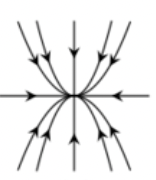
\includegraphics[scale = 0.9]{sink.png}
    \caption{A sink}
    \label{fig:my_label}
\end{figure}

\textbf{Case 2: both eigenvalues are positive: }\\
As we had concluded, our solution diverges away from the equilibrium point, due to exponential rise term. The equilibrium point is unstable, and is usually called a \emph{source}.

\begin{figure}[h]
    \centering
    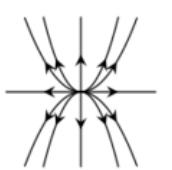
\includegraphics[scale = 0.9]{source.png}
    \caption{A source}
    \label{fig:my_label}
\end{figure}

\textbf{Case 3: eigenvalues have opposite signs: }\\
The solutions are a linear combination of exponential rise and decay terms. This, it will reach a minima(come close to the equilibrium point), and eventually the exponential rise term will cause it to diverge. The equilibrium point is unstable, and is called a \emph{saddle point}.
\begin{figure}[h]
    \centering
    
\includegraphics[scale = 0.9]{saddle.png}
    \caption{Saddle point}
    \label{fig:my_label}
\end{figure}

\textbf{Case 4: the eigenvalues are purely imaginary: }\\
The solutions are a linear combination of sines and cosines. They keep orbiting around the equilibrium point, neither converging, nor diverging. The equilibrium point is neturally stable, and is called a \emph{center}.

\begin{figure}[h]
    \centering
    
\includegraphics[scale = 1]{center.png}
    \caption{A center}
    \label{fig:my_label}
\end{figure}

\textbf{Case 5: complex eigenvalues with negative real part}\\
The solutions are a linear combination of exponentially decaying sinusoidal terms. The result is convergence to the equilibrium point, but the sinusoidal terms bring about oscillatory behavior. The combination of oscilation and exponential decay makes it look like a spiralling inward trajectory. Hence, the equilibrium point is said to be a \emph{spiral sink}

\begin{figure}[h]
    \centering
    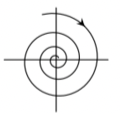
\includegraphics[scale = 0.9]{spiral_sink.png}
    \caption{A spiral sink}
    \label{fig:my_label}
\end{figure}

\textbf{Case 6: complex eigenvalues with positive real part}\\
A very similar case as the previous one, but now its a combination of exponentially growing sinusoids. The trajectory looks like an outward growing spiral. The equilibrium point is called a \emph{spiral source}.

\begin{figure}[h]
    \centering
    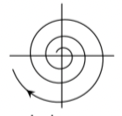
\includegraphics[scale = 0.9]{spiral_source.png}
    \caption{A spiral source}
    \label{fig:my_label}
\end{figure}



\subsection{Linearising a non-linear system of differential equations : The Jacobian matrix}
Consider the system of differential equations:
$$\frac{dx}{dt} = f(x, y)$$
$$\frac{dy}{dt} = g(x, y)$$
Let $(x_0, y_0)$ be a fixed point to this system. To see if it is stable, we have to linearise our system:
$$f(x, y) = f(x_0, y_0) + (x - x_0)\cdot f_x(x_0) + (y - y_0) \cdot f_y(y_0)$$
$$g(x, y) = g(x_0, y_0) + (x - x_0)\cdot g_x(x_0) + (y - y_0) \cdot g_y(y_0)$$
and since $(x_0, y_0)$ is a fixed point, $f(x_0, y_0) = g(x_0, y_0) = 0$.
\\
\\
Define a new set of variables, $u = x - x_0$ and $v = y - y_0$.
So, our linearised system becomes:
$$\frac{du}{dt} = u\cdot f_x(x_0) + v\cdot f_y(y_0)$$
$$\frac{dv}{dt} = u\cdot g_x(x_0) + v\cdot g_y(y_0)$$
\\
Hence, our coefficient matrix is
\begin{bmatrix}
f_x(x_0) & f_y(y_0)\\
g_x(x_0) & g_y(y_0)
\end{bmatrix}
, which is the Jacobian at $(x_0, y_0)$.
\\
\\
But we need to be careful in linearizing a system. Much like in the one variable analogue, where the case of $f'(x_0) = 0 $ wasn't enough to fully conclude the stability, a problem arises here too. A fixed point is said to be a hyperbolic/non-degenerate equilibrium, only when its Jacobian evaluated at that point has eigenvalues with non-zero real parts. A non-linear system is equivalent to its linearized counterpart for a hyperbolic equilibrium, but it is not necessarily so when it is degenerate. (for more details, refer to \texbf{Hartman-Grobman theorem}

\subsection{Stability of fixed points in the Lotka Volterra Model}
The Lotka-Volterra model has two fixed points:
\begin{itemize}
    \item The origin $(0, 0)$, which corresponds to extinction of both the species.
    \item The point in the first quadrant, $\left(\frac{c}{d}, \frac{a}{b} \right)$
\end{itemize}
\\
The Jacobian for our system is, \boldsymbol{J} = 
\begin{bmatrix}
a-by & -bx\\
dy & -c+dx
\end{bmatrix}, also called the Community Matrix.

\subsubsection{Stability of origin}
The Jacobian, evaluated at the origin equals
\begin{bmatrix}
a & 0\\
0 & -c
\end{bmatrix}, whose eigenvalues are $a$ and $-c$ (the eigenvalues of a diagonal matrix equal the diagonal elements itself). Since $a$ is positive, one of the eigenvalues is positive. This means that the origin is unstable.
\\
\\
Since it is unstable, points close to origin move further away. Physically this means that, even when the population levels are reduced to ridiculously low proportions, they will bounce back, according to this model. There is no way the populations can go extinct.
\\
\\
This is a flaw in our model, since populations can surely go extinct in real life. The idea that populations bounce back even after being nearly extinct is also a flaw, and this issue is commonly called "atto-fox problem", with the name arising from the fact that even when the predator/fox population is pushed to levels like $10^{-18}$ (1 atto), it still bounces back.

\subsubsection{Stability of the other point}
The Jacobian evaluated at $\left (\frac{c}{d}, \frac{a}{b} \right ) $ is 
\begin{bmatrix}
0 & \frac{-bc}{d} \\
\frac{ad}{b} & 0
\end{bmatrix},
and its eigenvalues are $i \sqrt{ac}$ and $-i \sqrt{ac}$, which are purely imaginary. When we solve using our matrix exponential, we see that the phase trajectories near this point are ellipses, centered around this point. This point acts as the center for trajectories. Since the nearby trajectories do not diverge, this is not an unstable equilibrium.
\\
\\

\href{https://drive.google.com/file/d/1GlrBvdVxhig_uhLE4dEE_yyL_uMg9w2e/view?usp=sharing}{Link to proof that trajectories close to the fixed point are ellipses.}


\section{Phase portrait of the Lotka Volterra model}

While an analytical solution to $x(t)$ and $y(t)$ is not easy, we can analyse the phase portrait of this system, i.e $y$ versus $x$.
\\
\\
Divide equation $(2)$ by $(1)$, to get :
$$\frac{dy}{dx} = \frac{y \cdot (-c + dx)}{x \cdot (a - by)}$$
\\
Separating variables, we get :
$$\left (\frac{a}{y} - b \right)dy = \left(\frac{-c}{x} + d \right)dx$$
\\
Integrate both sides to finally get : 
$$dx + by - c\cdot ln(x) - a\cdot ln(y) = E,$$
where E is a constant of integration, determined by our initial conditions.
\\
\\
So, if we let $f(x, y) = dx + by - c\cdot ln(x) - a\cdot ln(y)$, then our phase-space trajectories are the level curves of f(x, y). We have already established that solutions near the center have an elliptic phase trajectory, and hence are periodic (due to closed-ness of an ellipse). It turns out that all solutions to our model are in fact, periodic, and we are going to prove that this is the case.
\\
\\
We impose the conditions that $x \geq 0$ and $y \geq 0$, since prey and predator count cannot become negative.
\subsection{Nullclines}
Consider the system of differential equations:
\begin{align*}
   x_1' &= f_1(x_1, x_2, ..., x_n)\\
   x_2' &= f_2(x_1, x_2, ..., x_n)\\
   &\vdots \\
   x_n' &= f_n(x_1, x_2, ..., x_n)
\end{align*}
The $j^{th}$ nullcline of the system is the set of points such that $x_j' = 0$.
\\
\\
The nullclines for the Lotka Volterra equation are
\begin{itemize}
    \item $x = 0$ and $y = \frac{a}{b}$, the nullclines for x.
    \item $y = 0$ and $x = \frac{c}{d}$, the nullclines for y.
\end{itemize}

The nullclines $x = 0$ and $y = 0$ are invariant, i.e, the solutions $x = 0$ and $y = 0$ continue to stay there (in case of $x = 0$, y will exponentially decay and eventually, the solution converges to the origin, while for $y = 0$, x keeps rising exponentially, with y staying zero). However, the other two nullclines are not invariant, and solutions which cross these nullclines do not stay there.
\\

The nullclines divide the first quadrant into 4 regions as shown below:
\\
\\

\begin{figure}
    \centering
    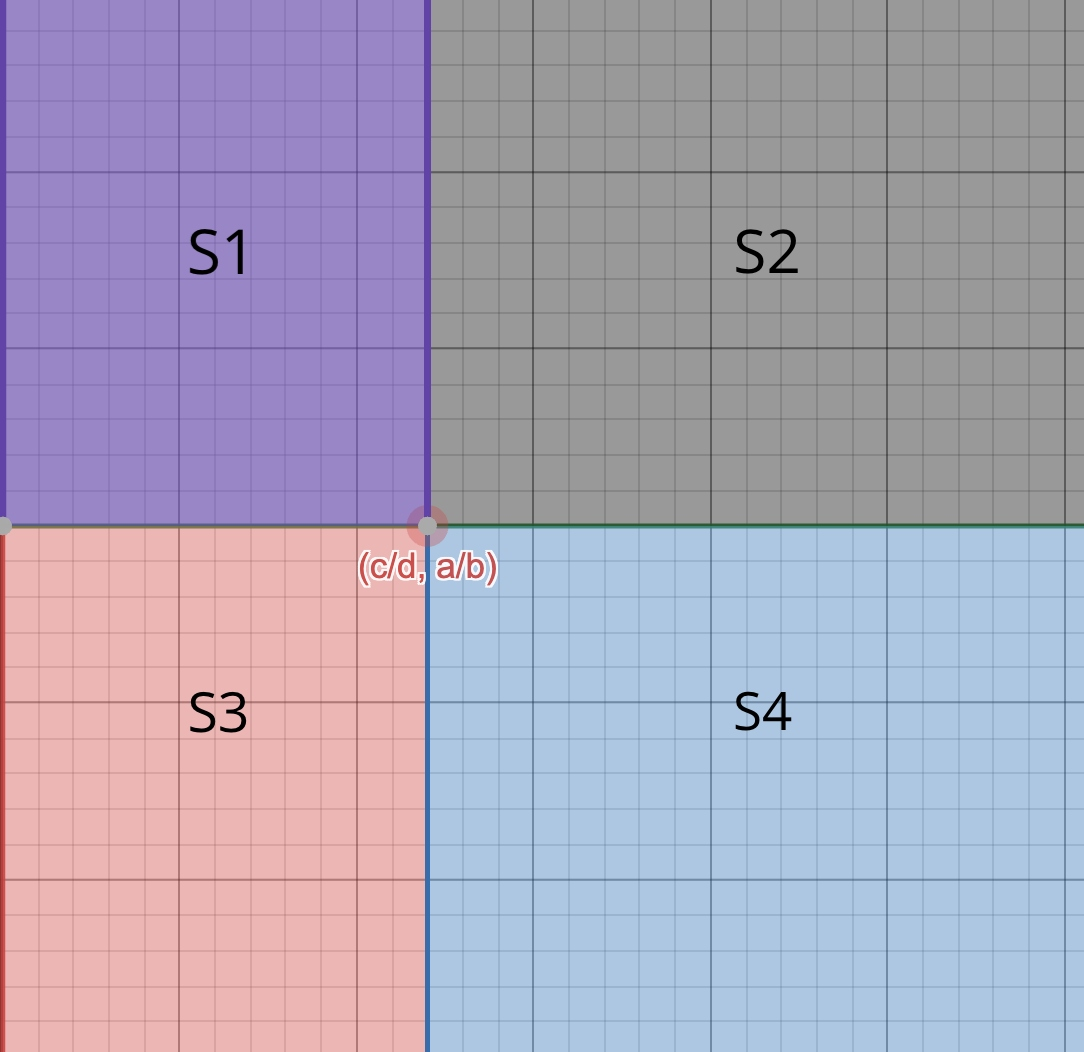
\includegraphics[scale = 0.7]{nullclines.jpg}
    \caption{}
    \label{}
\end{figure}
\\
\begin{itemize}
    \item In $S_1$, we have $x' < 0$ and $y' < 0$. This represents both population levels declining. 
    \item In $S_2$, we have $x' < 0$ and $y' > 0.$ The prey population declines, while the predator thrives.
    \item In $S_3$, we have $x' > 0$ and $y' < 0$. The predator declines, and the prey thrives.
    \item In $S_4$, we have both $x'$ and $y'$ greater than zero. Both population levels increase.
\end{itemize}
\subsection{Closedness of phase trajectories}
We make the claim that any phase trajectory that does not include our equilibrium point $\left(\frac{c}{d}, \frac{a}{b} \right)$ cannot stop abruptly at a point. If it did, then that point will be also be an equilibrium point, since our system doesn't evolve after that. This is an apparent contradiction since there is only one equilibrium point. So, our phase trajectory cannot just abruptly stop.
\\
\\
The phase trajectory cannot simply oscillate between two extremes either. If it did, it should have either $x' = 0$ or $y' = 0$ at both ends of its extremes (depending on which axis it oscillates about). But since there is only one nullcline, this cannot happen either. 
\\
\\
\\
Also, the phase trajectory cannot move back and forth along a curve like in the example below\\
\begin{figure}[h]
    \centering
    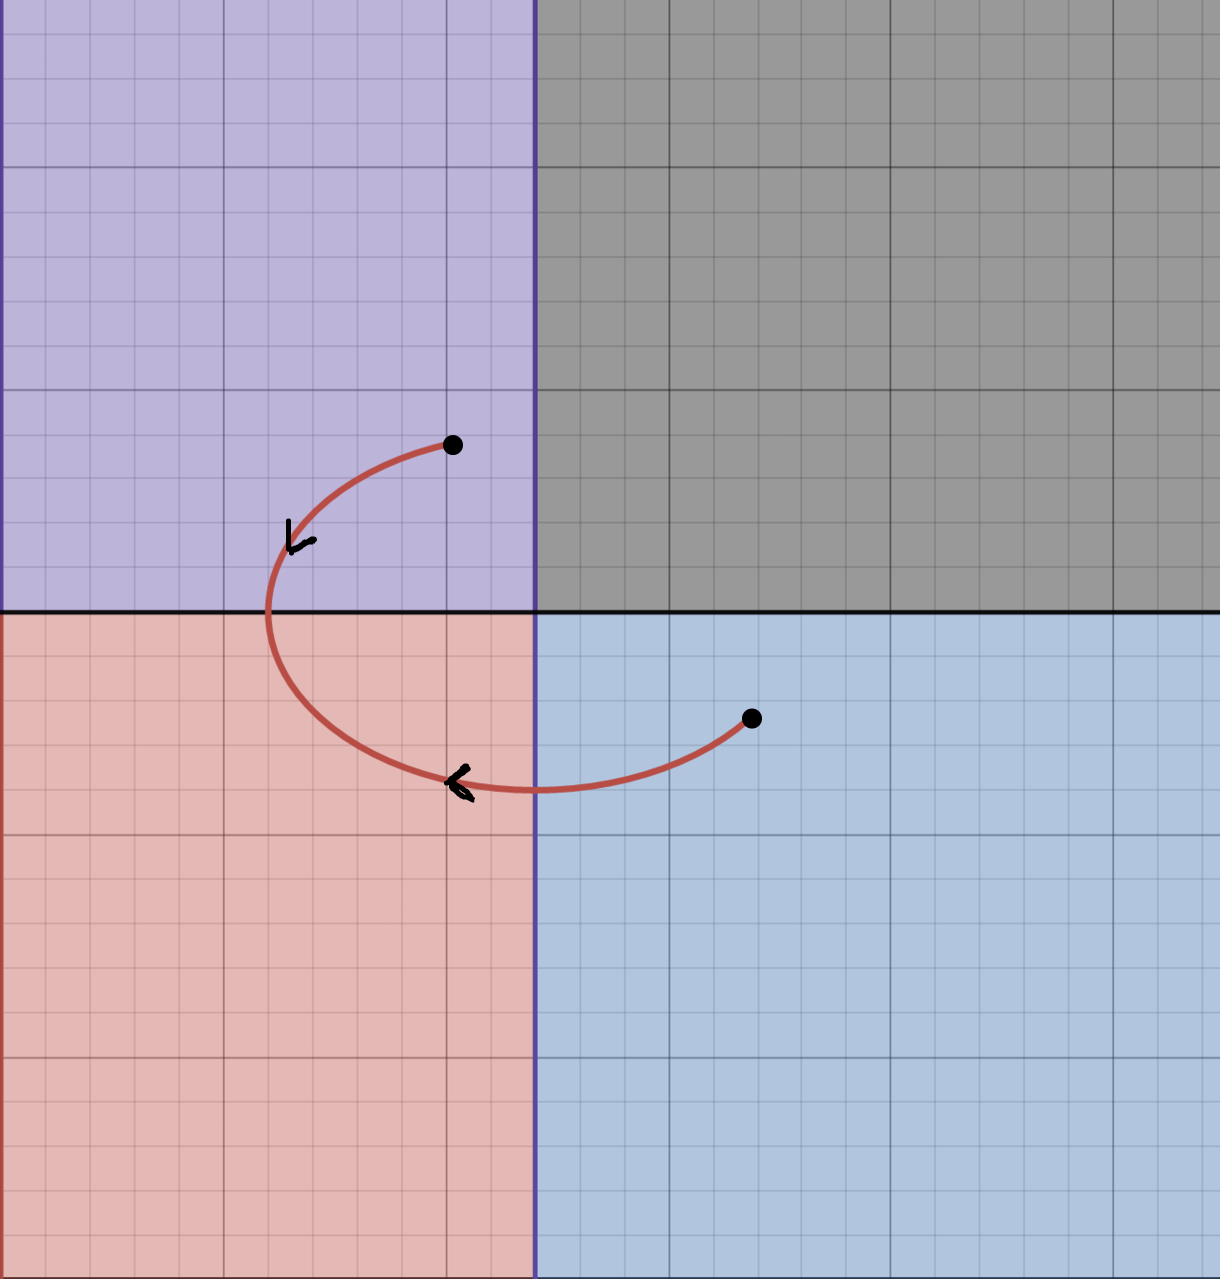
\includegraphics[scale = 0.15]{reverse_direction.png}
        \caption{Retracing itself, by reversing its direction is not possible.}
    \label{fig:my_label}
\end{figure}
\\
This is because, in each of the four sections, the curve moves only in 1 specific direction, due to the signs of $x'$ and $y'$. 
\begin{itemize}
    \item A solution in $S_3$ would move right and downward, since $x' > 0$ and $y' < 0$.
    \item A solution in $S_4$ can only move right and upward, since both $x'$ and $y'$ are positive.
    \item A solution in $S_2$ can only move left and upward, since $x' < 0$ and $y' > 0$.
    \item A solution in $S_1$ can only move left and downward, since both $x'$ and $y'$ are negative.
\end{itemize}
So, our solution cannot abruptly change its direction like this, since it is allowed to move only in specific ways. 
\\
\\Another way to reinforce this argument is that, since both $x(t)$ and $y(t)$ have continuous derivatives (due to the structure of our differential equation), the parametrization $(x(t), y(t))$ is a smooth one. Hence, our phase curve is also smooth. Due to smoothness, it cannot just retrace its path as shown.
\\
\\
We now claim and prove that any phase trajectory, with $x, y > 0$ is bounded (the cases of $x. = 0$ and $y = 0$ were already analysed):
\\
We know that our phase trajectories are level curves of $dx + by - c\cdot ln(x) - a\cdot ln(y)$, or that this value is a constant.\\
Regroup it as $(dx - c\cdot ln(x)) + (by - a\cdot ln(y)) = F(x) + G(y)$, where
$$F(x) = dx - c\cdot ln(x)$$
$$G(y) = by - a\cdot ln(y)$$
Now, we claim that any unboundedness can only be due to asymptotes, and that asymptotes are possible only in regions $S_2$ and $S_4$, if at all they exist:
\begin{itemize}
    \item In $S_3$, there is no possibility of unboundedness, since it in itself is a bounded set. A solution in $S_3$ also cannot ever enter the x-axis ($y=0$). Because, if it did, our conserved quantity will tend to infinity (since y $\to zero$, $-ln(y) \to \inf$), while initially our conserved quantity was finite. So, it cannot enter the x-axis, since a change in conserved quantity is forbidden. Hence, $y$ decreases, and $x$ increases, till our solution enters $S_4$
    \item A solution in $S_1$ eventually will have to enter $S_3$ only, since both $x$ and $y$ decrease in the region $S_1$. By a similar reasoning given to the solutions in $S_3$, a solution in $S_1$ too, cannot enter the y-axis. This, combined with fact that our phase curve cannot stop or retrace or oscillate forces the solution to enter $S_3$. 
    \item Solutions in $S_2$ have a decreasing $x$ and an increasing $y$. If we need unboundedness exists in $S_2$, it then has to satisfy this condition. Hence it can only be a vertical asymptote. 
    \item Similarly, in $S_4$, we can only have a horizontal asymptote.
\end{itemize}

\begin{figure}[h]
    \centering
    \begin{subfigure}[h]{0.4\textwidth}
        \centering
        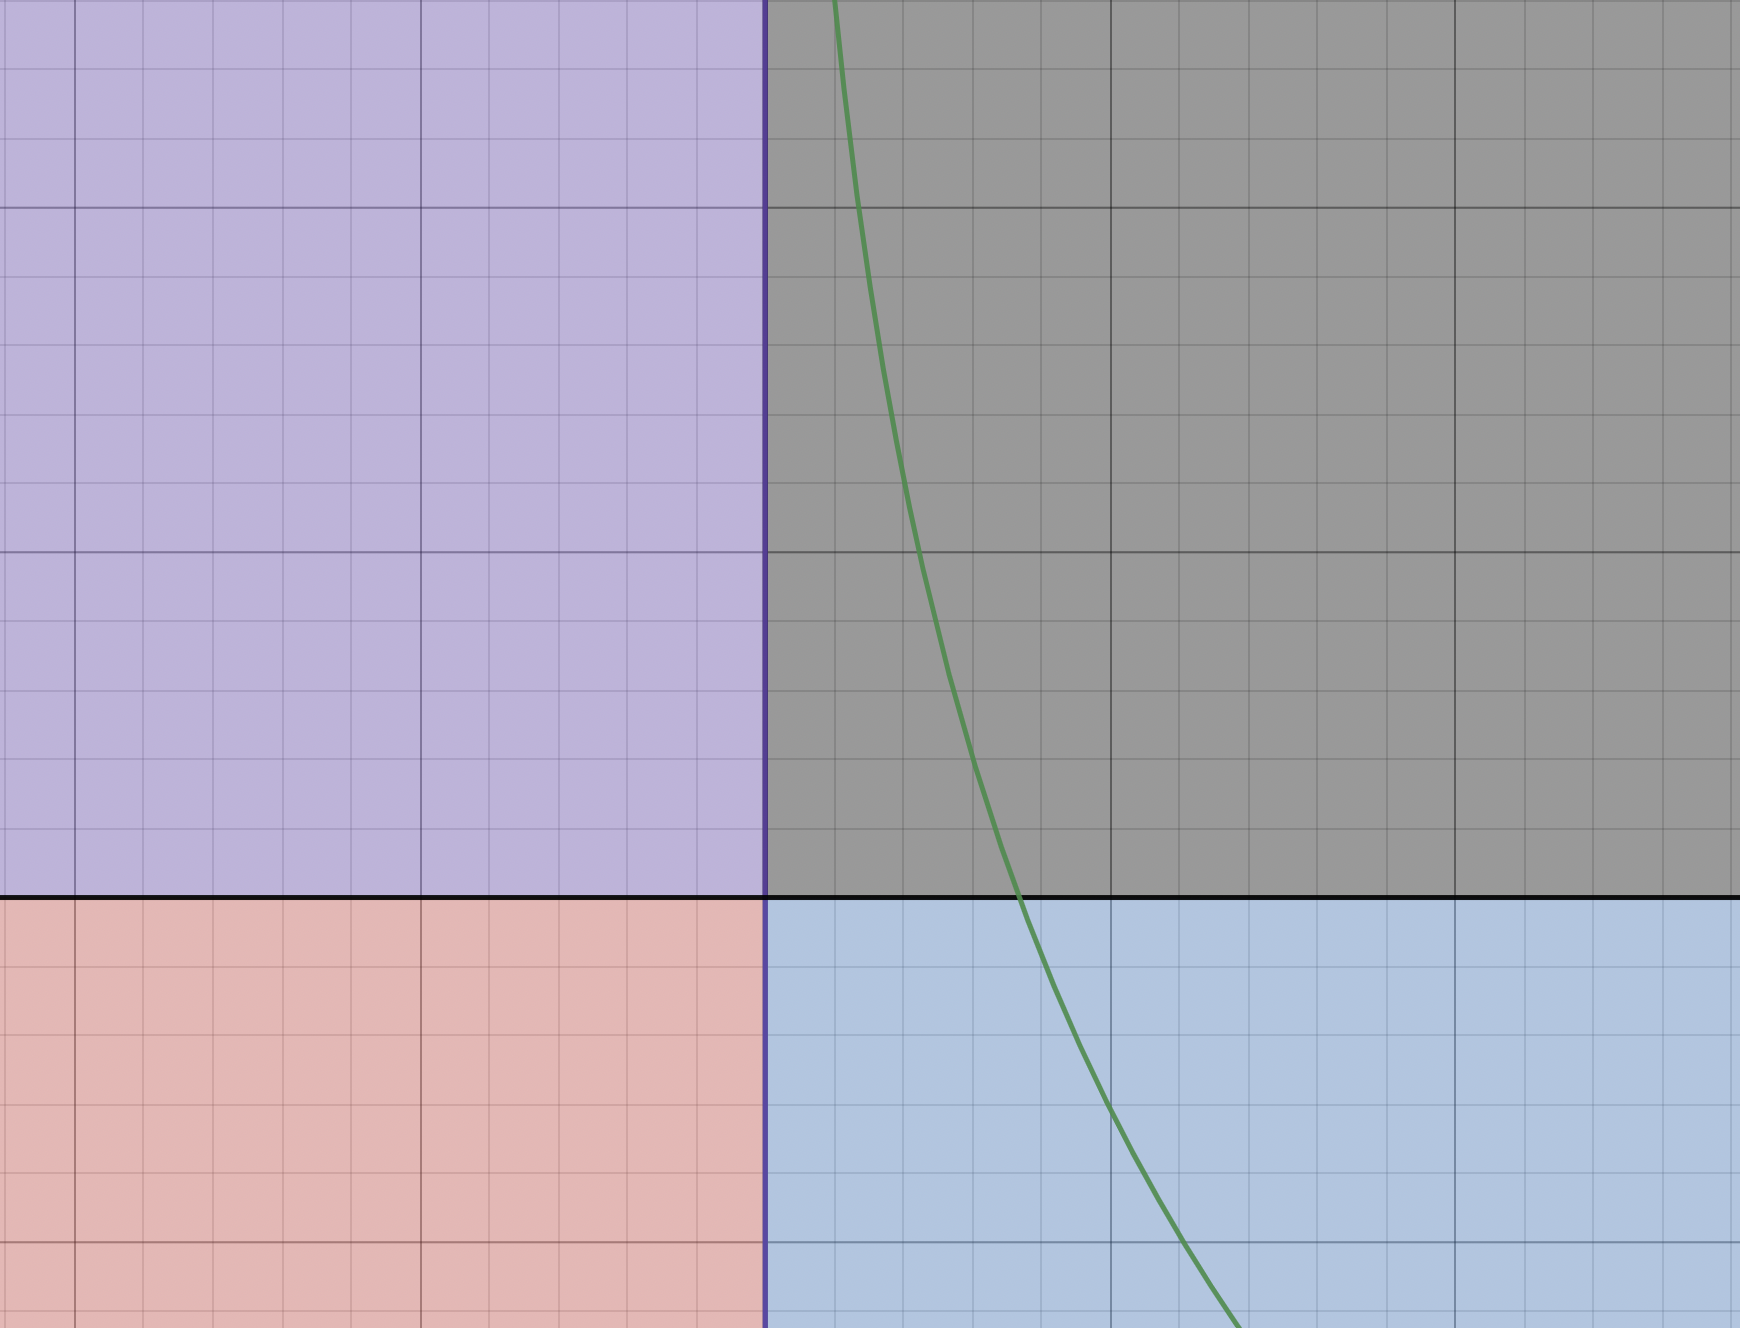
\includegraphics[width = \textwidth]{vertical.png}
        \caption{Veritcal asymptotes in $S_2$}
    \end{subfigure}
    \hfill
    \begin{subfigure}[h]{0.4\textwidth}
        \centering
        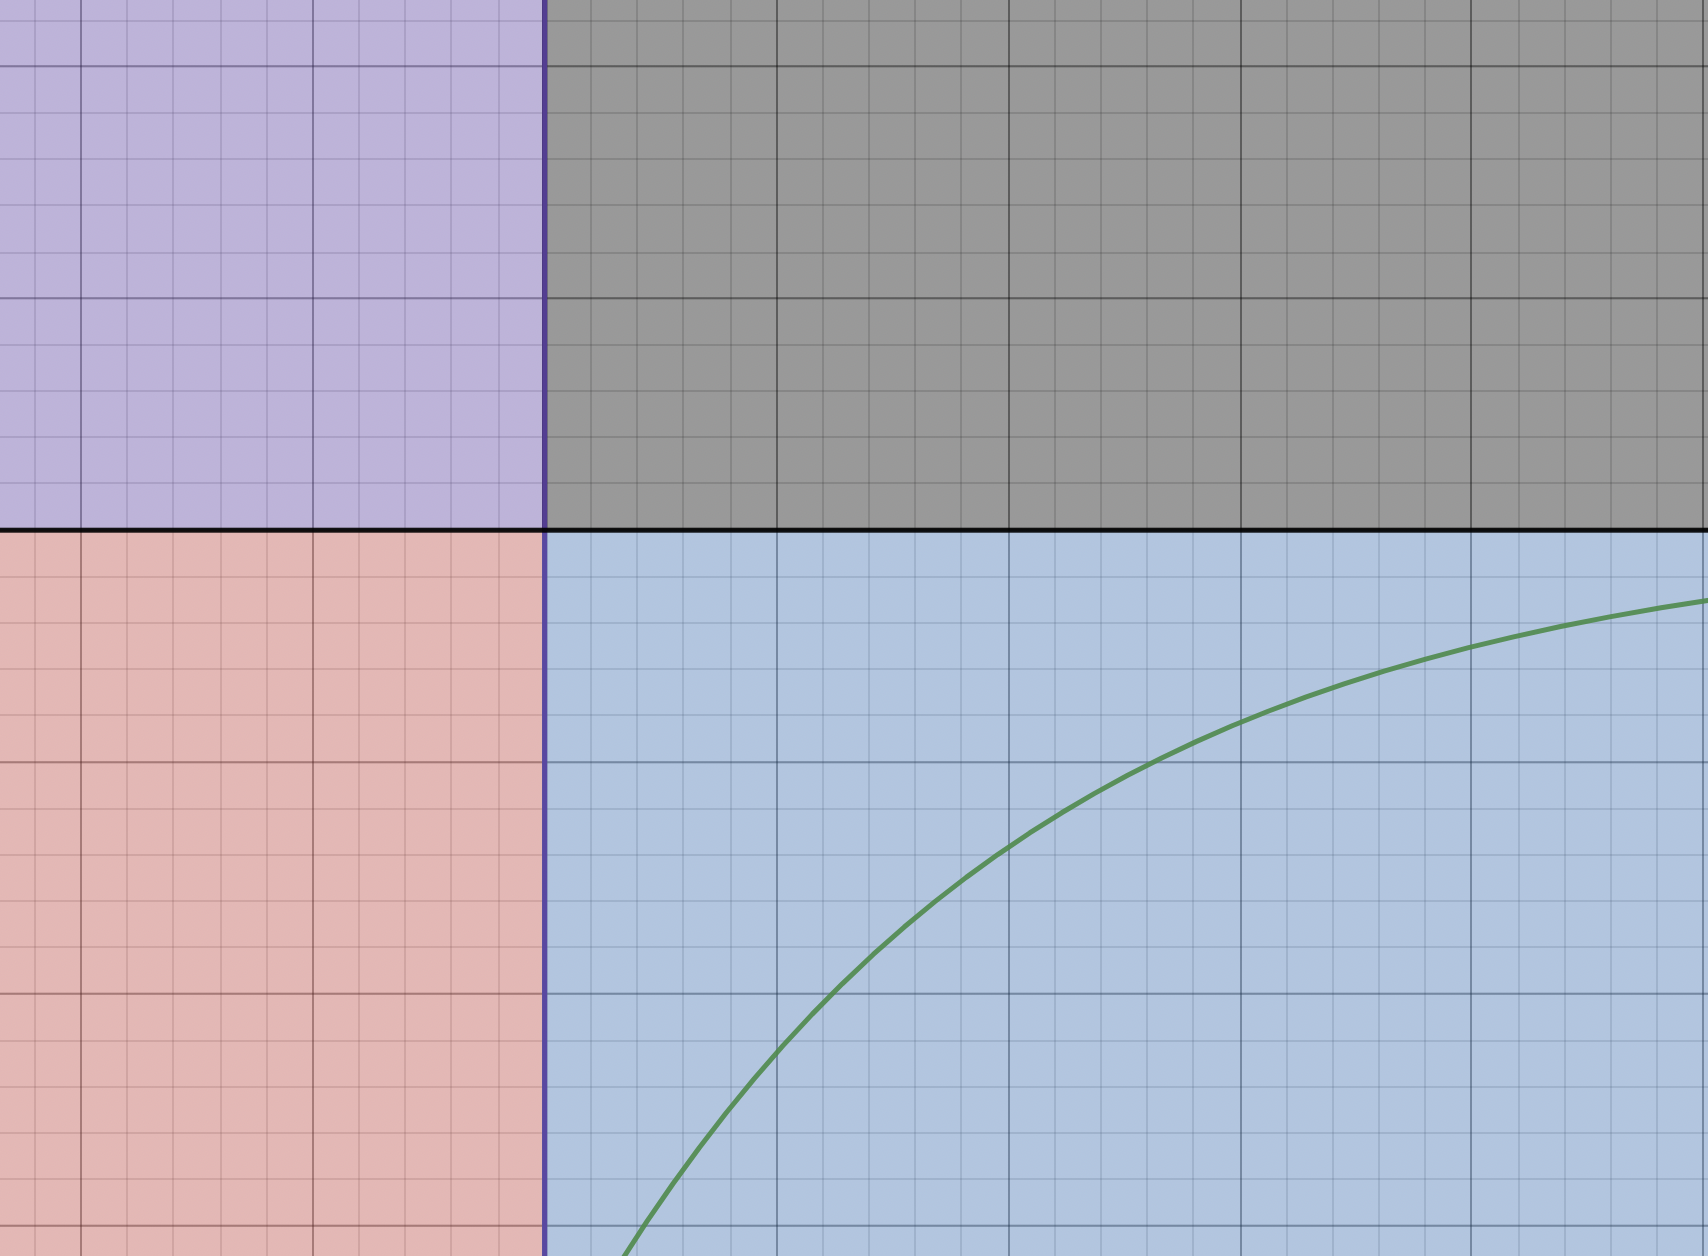
\includegraphics[width = \textwidth]{horizontal.png}
        \caption{Horizontal asymptotes in $S_4$}
    \end{subfigure}
\end{figure}
\\
\\
We now prove that asymptotes too, cannot exist. Without loss of generality, let us rule out the possibility of horizontal asymptote (vertical asymptote can be ruled out along similar lines):

First, observe that the function $F(x)$ and $G(y)$ have their minima at $x = \frac{c}{d}$ and $y = \frac{a}{b}$. The functions are one-one at either side of the minima, and are strictly increasing (i.e from $\frac{c}{d}$ to 0 and $\frac{c}{d}$ to $\infty$, $F(x)$ increases. Similarly does $G(y)$.) 
\\
Let the horizontal asymptote be $y = q$. Now, consider a point on the asymptote $\left(x_0, q - \epsilon \right)$, and another point $\left(\lambda x_0, q - \frac{\epsilon}{2} \right)$, for 2 positive constants $\lambda$ and $\epsilon$. \\
\\
Since $q - \frac{\epsilon}{2}$ is nearer to the minima of $G(y)$ than $q - \epsilon$, $G(q - \frac{\epsilon}{2}) < G(q - \epsilon)$, as $G(y)$ is strictly increasing. Thus, if the total energy of the system is to remain constant at these two points, we need $F(\lambda x_0) > F(x_0)$, and hence $\lambda > 1$.
\\
\\
The total energy of the system at the first point is $$E_1 = (dx_0 - c\cdot ln(x_0)) + b(q - \epsilon) - a\cdot ln(q - \epsilon),$$
and at the second point is $$E_2 = (d\lambda x_0 - c\cdot ln(\lambda x_0)) + b\left (q - \frac{e}{2}\right ) - a\cdot ln\left (q - \frac{\epsilon}{2}\right )$$

The difference in total energy between these points is,
$$\Delta E = E_2 - E_1 = -c \cdot ln(\lambda) + \frac{b\epsilon}{2} + a\cdot ln(\frac{2q - 2\epsilon}{2q - \epsilon})$$.

Putting the limit $\epsilon \to 0$ since this is an asymptote, we get 
$$\Delta E = -c \cdot ln(\lambda)$$
(A case to worry about would be to consider what if $\lambda$ too tends to 1. But that will not be the case for an asymptote, so we can safely ignore the terms containing $\epsilon$.)

We see that $\Delta E$ is not zero. There is an energy difference across an asymptote. Hence, asymptotes are not possible either.
\\
\\
After ruling out asymptotes, we then see that:
\begin{itemize}
    \item A solution starting in $S_3$, will move to $S_4$.
    \item A solution in $S_4$ will move to $S_2$.
    \item A solution in $S_2$ will move to $S_1$.
    \item A solution in $S_1$ will move to $S_3$.
\end{itemize}
\\
All these are due to the signs of $x'$ and $y'$ in the respective regions and the ruling out of pathological cases like converging to either axes/asymptotes/abrupt changes in trajectory.
\\
\\
So, we can see that a solution starting out in any of the 4 regions comes back to the same region. If we can prove that it returns to the same point it started, then we can conclude that it is a closed curve. 
\\
\\
Assume that our solution starts from the nullcline $y = \frac{a}{b}$, as shown:
\begin{figure}[h]
    \centering
    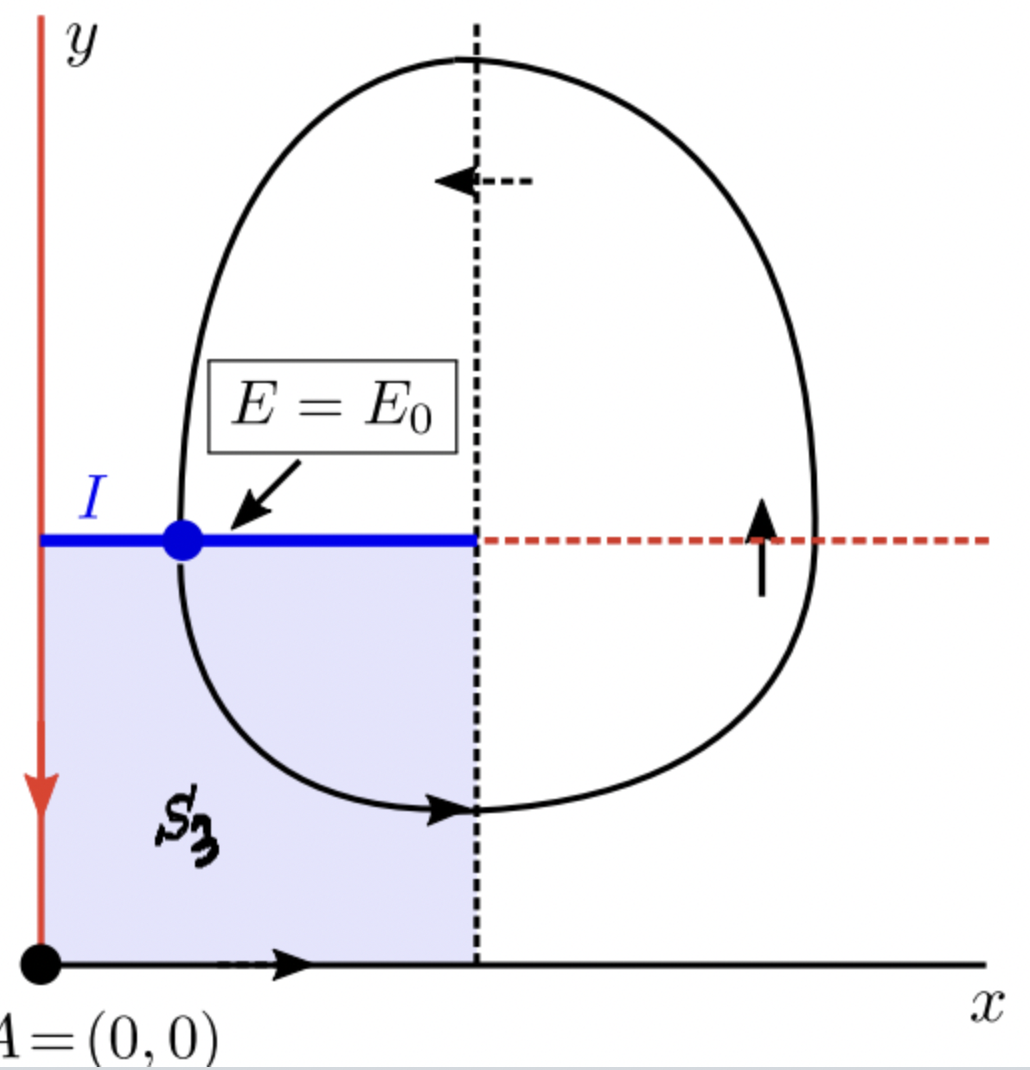
\includegraphics[scale = 0.3]{closedness.png}
    \caption{}
    \label{fig:my_label}
\end{figure}
\\
\\
The solution then moves to $S_3$, goes to $S_4$, then $S_2$, then $S_1$ and then returns back to the nullcline shown in bold blue. 
\\
\\
Since the equation of the nullcline is $y = \frac{a}{b}$, the value of $y$ is fixed. And we know that our function $F(x) = dx - c\cdot ln(x)$ is strictly decreasing from 0 to $\frac{c}{d}$. So, $F(x)$, and hence total energy is a one-one function in the nullcline shown in bold. So, if our total energy is to remain constant, it must come back again to the same point, $I$. 
\\This completes our proof that phase trajectory is closed.
\\
\\
The phase trajectory intersects itself/it is closed. We proved this by saying that the starting and end point, $I$ is the same. But since this system is autonomous, we can say more : the solution is actually periodic as well! While a periodic solution trivially implies a closed phase trajectory, the converse is not so trivial, and is in general, not true for non-autonomous system (systems where there is explicit time dependence in our differential equations).
\\
\\


\subsection{Periodic oscillations from closed trajectories}

Consider the autonomous system:
$$\frac{dx}{dt} = f(x, y)$$
$$\frac{dy}{dt} = g(x, y),$$
with the initial conditions $x(a) = x_0$ and $y(a) = y_0$, along with self-intersection after some time point $x(a + P) = x(a) = x_0$, $y(a + P) = y(a) = y_0$, for some $P$.

To prove that the solution is periodic, consider a new set of functions $x_1(t) = x(t + P)$ and $y_1(t) = y(t + P)$. These two solutions obey the equations:
$$\frac{dx_1}{dt} = f(x(t + P), y(t + P))$$
$$\frac{dy_1}{dt} = g(x(t+P), y(t+P))$$

Again, substitute for $x(t + P)$ and $y(t + P)$ in the right hand side:
$$\frac{dx_1}{dt} = f(x_1(t), y_1(t))$$
$$\frac{dy_1}{dt} = g(x_1(t), y_1(t))$$.

Our initial conditions are $x_1(a) = x(a + P)$, which we know to be $x_0$ and $y_1(a) = y(a + P)$, which is also $y_0$.
\\
\\
So, ($x$, $y$) and ($x_1$, $y_1$) both obey the same set of differential equations, with the same initial conditions. By the uniqueness theorem, our solutions must also be the same.
\\
\\
Hence $x_1(t) = x(t)$ or $x(t+P) = x(t)$ for all t, and $y_1(t) = y(t)$ or $y(t + P) = y(t)$, for all t. Our solutions are periodic with period $P$. However, we cannot determine the fundamental period from this.
\\
\\
It is clear that closed trajectory need not imply periodicity for a non-autonomous system. For a non-autonomous system, our equations for $x_1$ and $y_1$ would be 
$$\frac{dx_1}{dt} = f(x_1(t), y_1(t), t +P)$$
$$\frac{dy_1}{dt} = g(x_1(t), y_1(t), t + P),$$ and hence our R.H.S is no longer the same.


\subsection{Invariance of autonomous systems to time shifts}

All autonomous systems are time invariant. That is, if $(x(t), y(t))$ is a solution to the above system, then so is $(x(t+ \tau), y(t + \tau))$ for any $\tau$.
\\
\\
To realize this, replace $t$ by $t + \tau$ in our system of differential equations :
$$\frac{dx(t+\tau)}{dt} =f\left (x(t+\tau), y(t+\tau)\right )$$
$$\frac{dy(t+\tau)}{dt} = g(x(t+\tau), y(t+\tau))$$

Define $x_1(t) = x(t+\tau)$ and $y_1(t) = y(t+\tau)$. Then, we get:

$$\frac{dx_1}{dt} = f(x_1, y_1)$$
$$\frac{dy_1}{dt} = g(x_1, y_1)$$


Thus $(x_1(t), y_1(t))$ also solves the system of equation. Hence $x(t+\tau), y(t+\tau))$ is also a solution.
\\
\\
If the original solution has the initial conditions $(x(t_0), y(t_0)) = (x_0, y_0)$, then a translated solution will have the initial condition $(x_1(t_0 - \tau), y_1(t_0 - \tau)) = (x_0, y_0)$.
\\
\\ 
Since in autonomous systems, the evolution is governed only by the coordinates at present (and importantly, not by time), the translated solution will also follow the same phase trajectory as the original solution, but will always be $\tau$ seconds ahead.
\\
\\
So, every phase trajectory represents infinitely many solutions, each differing from one another only by a shift in time.

\subsection{Unique, non-intersecting phase trajectories}

No two different phase trajectories of an autonomous system can intersect one another. 
\\
\\
Let $(x_1(t), y_1(t))$ and $(x_2(t), y_2(t))$ be two solutions to our system of equations, with an apparent intersection : $$(x_1(a), y_1(a)) = (x_2(b), y_2(b)) = (x_0, y_0)$$
\\
\\
Consider the pair of functions $$(x_3(t), y_3(t)) = (x_2(t+b-a), y_2(t+b-a)) \text{, a time-translated version }$$ $(x_2(t), y_2(t))$. 
\\
\\
By our previous arguments, $(x_3(t), y_3(t))$ also solve for the system of differential equations. Observe that:
$$x_3(a) = x_2(a + b - a) = x_2(b) = x_0 \text{and}$$
$$y_3(a) = y_2(a + b - a) = y_2(b) = y_0.$$

So $(x_3, y_3)$ and $(x_1, y_1)$ also have the same initial conditions. Therefore, by the uniqueness theorem, they are identical solutions, and hence have the same phase trajectories.
\\
\\
But since $(x_3, y_3)$ is just a time-translation if $(x_2, y_2)$, their trajectories are coincident too. This means the trajectories of our two solutions are identical. (in fact, we can use a similar argument to state at $x_2(t) = x_1(t + a - b)$ and $y_2(t) = y_1(t + a - b)$).
\\
\\
Thus, any pair of phase trajectories are either completely coincident, or they never intersect.
\\
\\
This means that the trajectories of the Volterra model are non-intersecting closed loops, similar to the rings in a tree trunk.

\begin{figure}[h]
    \centering
    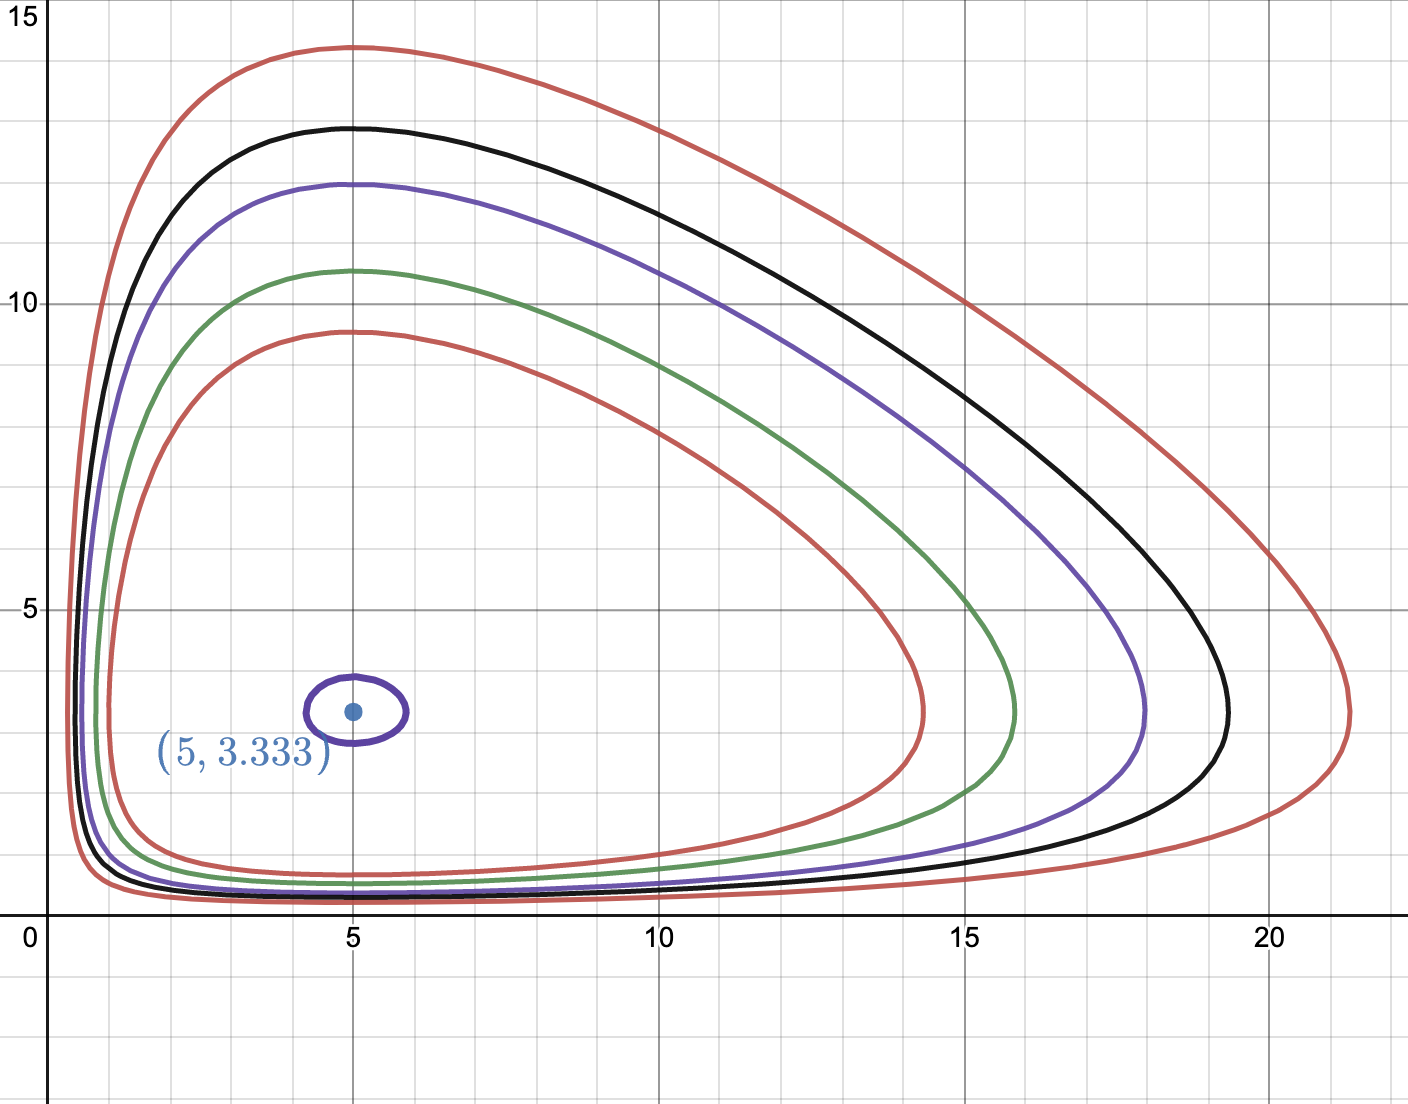
\includegraphics[width = 0.8\textwidth]{phase.png}
    \caption{Different phase trajectories for $a = 1$, $b = 0.3$, $c =1$ and $d = 0.2$}
    \label{}
\end{figure}


\section{Variants of the Lotka Volterra Model:}

We stumbled upon the flaw that no species can go extinct in this model, even when pushed to unrealistically low proportions. So we can try coming up with better alternatives, and we start off with the simplest correction, \textbf{the logistic growth}.

\subsection{Limited grass and competition between the prey}
One of the major flaws in our model was to let the prey grow exponentially, when left unchecked. But this is not a realistic assumption, as the total resources available is finite.
\\
\\
The preys have to compete with one another to consume the sparse resources. To include the effect of this intra-specific competition, we modify our equation (rate of change of prey, when left unchecked) to:
$$\frac{dx}{dt} = \alpha x \left (1 - \frac{x}{K}\right )$$
\\
In such a case, $x(t)$ has the solution $$x(t) = \frac{K\cdot Ae^{\alpha t}}{1 + A e^{\alpha t}} \text{ ,}$$
 where A is an appropriate constant
\\
\\
Thus, in the limit $t \to \infty$, $x(t) \to K$, and hence the logistic growth model allows only finite levels of populations. 
\\
\\
This suggests that using the logistic growth for the prey population is a good idea, since it doesn't allow for unrestricted growth.

\subsection{Logistic growth for prey}
So, we model our system of differential equations as :
$$\frac{dx}{dt} = ax\left(1 - \frac{x}{K}\right) - bxy$$
$$\frac{dy}{dt} = -cy + dxy$$

Such a model has three equilibrium points:
\begin{itemize}
    \item $(0, 0)$, extinction of both species.
    \item $(K, 0)$, the prey has reached its maximum/\emph{carrying capacity}, while the predator goes extinct.
    \item $\left(\frac{c}{d}, \frac{a}{b} \left(1 - \frac{c}{Kd} \right) \right)$, which corresponds to mutual existece of both the species. (provided $K > \frac{c}{d}$) 
\end{itemize}

\subsection{Analysis of equilibrium points:}

The Jacobian matrix for the system is 
\begin{bmatrix}
a - \frac{2ax}{K} - by & -bx\\
dy & -c + dx
\end{bmatrix}
\\

\begin{itemize}
    \item At the origin, the Jacobian equals 
    \begin{bmatrix}
    a & 0\\
    0 & -c
    \end{bmatrix}, whose eigenvalues are $a$ and $-c$. Thus the origin/mutual extinction is a saddle point.
    \item At the point $(K, 0)$, the Jacobian equals 
    \begin{bmatrix}
    -a & -Kb\\
    0 & -c + Kd
    \end{bmatrix}.
    Two cases arise, depending on whether $K$ is greater or less than $\frac{c}{d}$.
    \\
    \\
    If $K < \frac{c}{d}$, then both the eigenvalues are negative, and hence this is a stable point. In this case, the predator population dies out early on, and beyond that, the prey population grows logistically, converging to its carrying capacity.
    \\
    \\
    If $K > \frac{c}{d}$, then this point is a saddle, as the eigenvalue $-c + Kd$ is greater than 0.
    \item At the third equilibrium point, the Jacobian equals 
    \begin{bmatrix}
    \frac{-ac}{Kd} & \frac{-bc}{d}\\
    \frac{ad}{b} \left(1 - \frac{c}{Kd} \right) & 0
    \end{bmatrix}
     and its eigenvalues depend on the relative magnitudes of $a$, $c$ and $\frac{c}{Kd}$. But we can perform analysis in the limit:
    \\
    \\
    For $K \to \frac{c}{d}^{+}$, the eigenvalues are approximately $-a$ and $0$. Hence, this point is expected to be stable. Physically, since the carrying capacity is low (just above its min value), this point corresponds to very low predator populations $\left(\text{due to the } 1 - \frac{c}{Kd} \text{term } \right).$
    \\
    \\
    For the limit $K \to \infty$, this point has purely imaginary eigenvalues, and hence acts as a center. This makes sense, as the above limit means that the carrying capacity is very large, which boils down to our usual Lotka-Volterra model.
    \end{itemize}
\subsection{Phase trajectory}
Since the stability of one of our points depends on the relative values of certain parameters, its not possible to draw a general phase trajectory.
\\
Below is the phase trajectory, for the paramteters $a = 5$,  $b = 1$, $c = 2$, $d = 1$ and $K = 5$.

\begin{itemize}
    \item The origin has eigenvalues of $5$ and $-2$, and is therefore a saddle point.
    \item The point $(5, 0)$ has eigenvalues $-5$ and $3$, and is also a saddle point.
    \item The point $(2, 3)$ has the eigenvalues $-1 \pm i\sqrt{5}$. It a stable spiral sink
\end{itemize}

\begin{figure}[h]
    \centering
    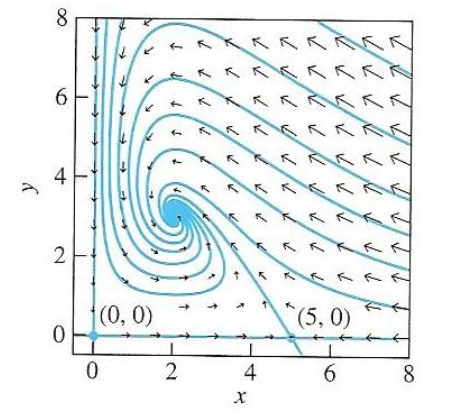
\includegraphics[scale = 0.9]{logistic_grow.png}
    \caption{}
    \label{fig:my_label}
\end{figure}

\subsection{Competition in predator:}
We can also bring about predator-predator intraspecific competition, by incorporating a similar $-y^2$ term in our governing equations:
$$\frac{dx}{dt} = ax\left (1 - \frac{x}{K_1}\right) - bxy$$
$$\frac{dy}{dt} = -cy\left(1 + \frac{y}{K_2}\right) + dxy$$

\subsection{An interesting case : two species competing for the same resource}

We could also have an ecosystem with two preys, like rabbits and sheep, where none benefits at the expense of the other, yet, the existence of one has a detrimental effect on the existence of the other.

The population of the two species are modelled as:
$$\frac{dx}{dt} = r_1x \left(\frac{K_1 - x - \beta_1 y}{K_1}\right)$$
$$\frac{dy}{dt} = r_2y \left(\frac{K_2 - y - \beta_2 x}{K_2}\right)$$
\\
\\
\textbf{What do $\beta_1$ and $\beta_2$ represent?}\\
A high value of $\beta_1$ would mean that the effect of the second species on the survival of the first is quite high. Even a low number of the second species will inhibit the growth rate of the first to a great extent.\\
Similarly, a high value of $\beta_2$ means that the effect of the first species on the growth rate of second is high.\\
Low values of $\beta$ represent low effects and $\beta_1 = \beta_2 = 0$ means that the two populations have no effect on one other - both just have independent, logistic growths.

\subsubsection{Equilibrium points and stability analysis:}

We have four equilibrium points in this system:
\begin{itemize}
    \item $(0, 0)$, total extinction
    \item $(K_1, 0)$, extinction of second species
    \item $(0, K_2)$, extinction of first species
    \item $\left(\frac{K_1 - K_2\beta_1}{1 - \beta_1\beta_2}, \frac{K_2 - K_1\beta_2}{1 - \beta_1\beta_2} \right)$, co-existence of both species (provided each expression is positive)
\end{itemize}

For the fourth point to lie in the first quadrant, we have two scenarios:
\begin{itemize}
    \item $\beta_1\beta_2 > 1$, in which case both $K_1 - K_2\beta_1$ and $K_2 - K_1\beta_2$ are negative. In this case, the product of the coefficients of interspecies competition is more than the product of coefficients of intraspecies competition/self-inhibition. Thus, we say that effect of competition is more than that of inhibition.
    \item $\beta_1\beta_2 < 1$, in which case both $K_1 - K_2\beta_1$ and $K_2 - K_1\beta_2$ are positive. Here, the effect of inhibition is more than that of competition.
\end{itemize}
\\
\\
\textbf{Case 1 : effect of competition is more than inhibition}\\
In this case, we have:
\begin{itemize}
    \item The origin to be an unstable source
    \item The points $(K_1, 0)$ and $(0, K_2)$ to be stable sinks.
    \item The other equilibrium point to be a unstable saddle.
\end{itemize}
\\
Thus, mutual existence is not a possibility, and 1 species is invariably driven to extinction. This should make sense, as the effect of interspecies competition is high. Total extinction, however, isn't a possibility
\\
\\
\textbf{Case 2 : effect of competition is less than inhibition}\\
In this case, we have:
\begin{itemize}
    \item The origin as an unstable source
    \item The points $(K_1, 0)$ and $(0, K_2)$ to be unstable sinks.
    \item The other equilibrium point to be a stable sink.
\end{itemize}
\\
Hence, in this case, mutual existence is the only possibility, and no species completely drives the other out. This too makes sense, as the effect of interspecific competition is low.

\section{Generalized Lotka-Volterra model}

The Lotka-Volterra model can be extended to an $n$-species ecosystem. Let $x_1$, $x_2$, ... $x_n$ represent the population levels of the $n$ species. They are governed by the equation:
$$\frac{dx_i}{dt} = x_i \cdot f_i(\overrightarrow{x})$$
where $f(\overrightarrow{x})$ is defined as:
$$f(\overrightarrow{x}) = \overrightarrow{r} + \boldsymbol{A}\overrightarrow{x}$$
where $\overrightarrow{r}$ is a constant vector, $\overrightarrow{x}$ is the vector field whose components are $x_1$, $x_2$, ... , $\boldsymbol{A}$ is a constant matrix and $f_i$ represents the $i^{th}$ component of f.
\\
\\
\textbf{What the vector $\overrightarrow{r}$ and the matrix A say?}
The value of $r_i$ described the intrinsic growth rate of the $i^{th}$ species. If it is positive, then the species is capable of reproducing even in the absence of other species (usually seen in case of plants). A negative value of $r_i$ means that the species cannot reproduce on its own, and has a natural death rate. This is the case on animals, prey or predator alike.
\\
\\
The value of $a_{ij}$ represents the effect of the $j^{th}$ species has on the $i^{th}$ species.

\begin{itemize}
    \item \textbf{Neutralism: } This is the case when $a_{ij} = a_{ji} = 0$. The two species have no direct influence on the other.
    \item \textbf{Amenalism: } This corresponds to $a_{ij} < 0$ but $a_{ji} = 0$. The $j^{th}$ species has a negative effect on the $i^{th}$ species, without getting any significant influence back.
    \item \textbf{Commenalism: } One species benefits, without affecting the other. Here, we have $a_{ij} > 0$ and $a_{ji} = 0$
    \item \textbf{Competition: } Each has a detrimental effect on the other. We have $a_{ij}, a_{ji} < 0$
    \item \texbf{Antagonism: } One species benefits at the expense of the other. We have $a_{ij} < 0$, and $a_{ji} > 0$. Such a relation is often called a prey-predator relation or a host-parasite relation.
    \item \textbf{Mutualism: } Each species benefits due to the existence of the other. Such a relation is also called a symbiotic relationship. Here $a_{ij}, a_{ji} > 0$
\end{itemize}

Additionally, usually $a_{ii} < 0$, due to the intraspecific competition in a species.

\section{Summary and conclusion}
Using the Lotka-Volterra model, we have studied the basics of stability theory, linearization and properties of autonomous systems, and applied it to our model in question.\\
We also analysed various other variants of the Lotka-Volterra model and studied how each parameter affects the relationship between the different species.

\section{References:}
\begin{itemize}
    \item \href{https://services.math.duke.edu/~jtwong/math356-2019/lectures/Dynamics4_cons_lyapunov.pdf}{https://services.math.duke.edu/~jtwong/math356-2019/lectures/Dynamics4_cons_lyapunov.pdf}
    \item \href{https://drive.google.com/file/d/1tboIZS9Yj1FpIMX4Jr3KekhGSQTwRQAy/view?usp=sharing}{https://drive.google.com/file/d/1tboIZS9Yj1FpIMX4Jr3KekhGSQTwRQAy/view?usp=sharing}
    \item \href{https://drive.google.com/file/d/1e35lx8tU4-clY7_LsaqUjppbndHJL37R/view?usp=sharing}{https://drive.google.com/file/d/1e35lx8tU4-clY7_LsaqUjppbndHJL37R/view?usp=sharing}
    \item \href{https://tinyurl.com/y7w4uhye}{https://tinyurl.com/y7w4uhye}
\end{itemize}
\end{document}
